\level{1}{Casi d'uso}
L’analisi del capitolato, l’incontro con il proponente e la discussione tra gli \insrole{Analisti} hanno portato all'individuazione dei casi d'uso riportati di seguito. 
I casi d'uso sono suddivisi in tre categorie, in quanto il progetto prevede la creazione di tre sistemi differenti:
\begin{description}
	\item[Norris] sono i casi d'uso inerenti alle funzionalità offerte dal framework;
	\item[Applicazione Android] sono i casi d'uso inerenti all'utilizzo dell'applicazione Android;
	\item[Dashboard] sono i casi d'uso inerenti all'utilizzo della dashboard.
\end{description}
Ogni caso d'uso è identificato da un codice univoco. La descrizione del modo in cui un caso d'uso viene identificato è rintracciabile nel documento \insdoc{Norme di Progetto v1.00}.\\
Si noti che nell'analisi dei casi d'uso viene utilizzato il concetto di attore. Un attore è qualsiasi cosa esterna al sistema che interagisca con esso. In particolare, un attore può rappresentare sia un utente umano sia un sistema esterno. È necessario dunque rimarcare che la differenza tra un attore e un utente è che il primo rappresenta il ruolo di un'entità esterna che interagisce con il sistema, mentre il secondo rappresenta in realtà una particolare classe di attori, quelli umani.\\
In seguito a queste considerazioni, è evidente come si debba mettere in relazione gli utenti descritti in precedenza con gli attori che vengono individuati nei casi d'uso espressi in seguito. Quindi, lo studio di ogni singolo sistema inizia con l'esplicazione della relazione che intercorre tra gli utenti e gli attori.

\level{2}{Norris}
	\level{3}{Relazione tra utenti e attori}
	Mettiamo in relazione gli utenti utilizzatori di Norris con gli attori che sono stati utilizzati nei seguenti casi d'uso. Si ricordi, infatti, che gli utenti non sono altro che una particolare classe degli attori.
	\begin{figure}[H]
		\centering
		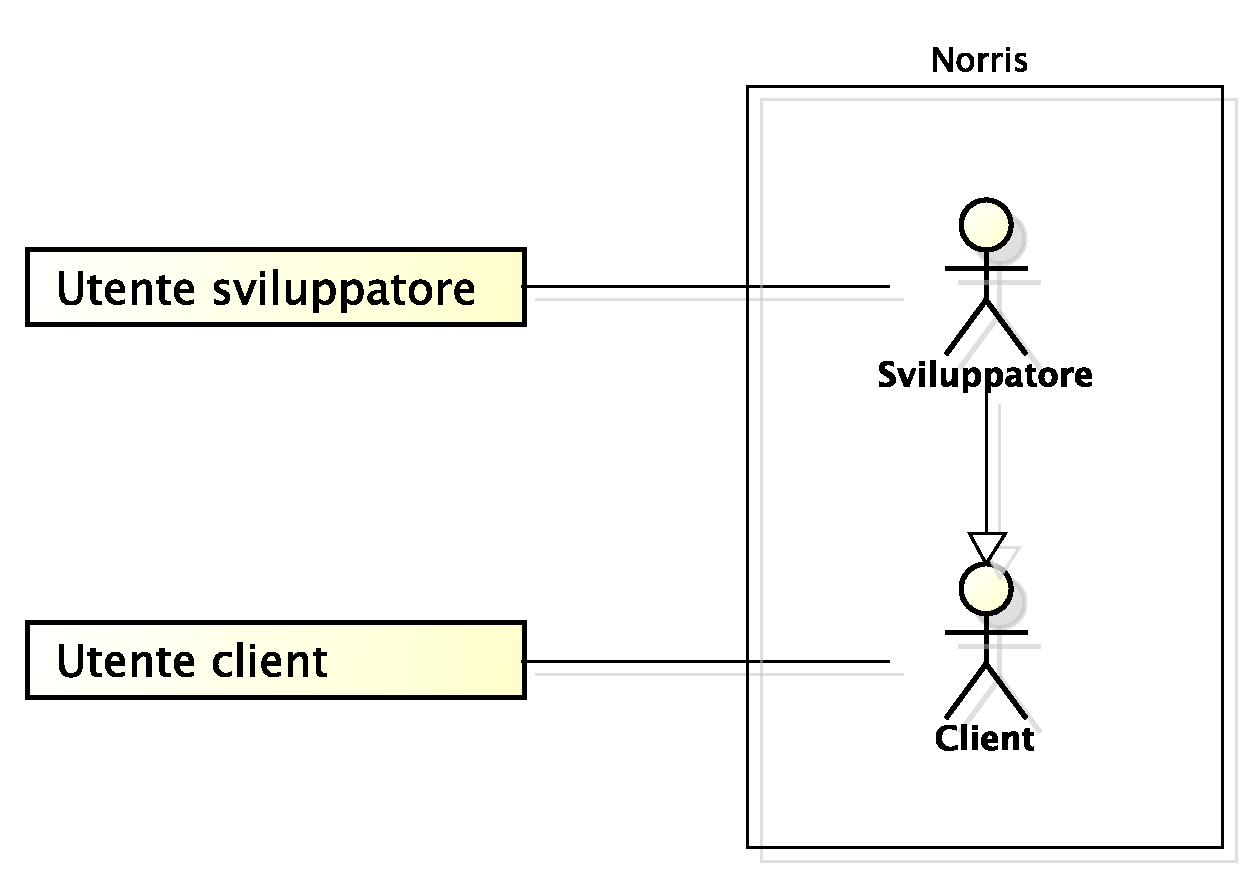
\includegraphics[scale=0.4]{Pics/UtentiAttoriNorris}
		\caption{Norris - Relazione tra utenti e attori}
	\end{figure}
	\input{UseCase/UCN.tex}

\level{2}{Applicazione Android}
	\level{3}{Relazione tra utenti e attori}
	Mettiamo in relazione gli utenti utilizzatori di dell'applicazione Android con gli attori che sono stati utilizzati nei seguenti casi d'uso. Si ricordi, infatti, che gli utenti non sono altro che una particolare classe degli attori.
	\begin{figure}[H]
		\centering
		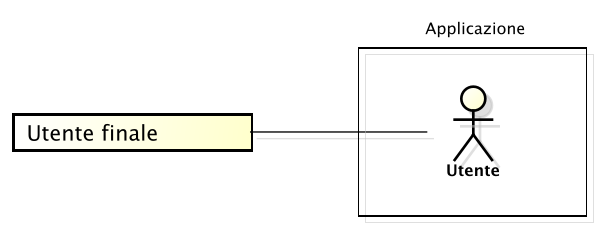
\includegraphics[scale=0.4]{Pics/UtentiAttoriApplicazione}
		\caption{Applicazione - Relazione tra utenti e attori}
	\end{figure}
	\input{UseCase/UCA.tex}

\level{2}{Dashboard}
	\level{3}{Relazione tra utenti e attori}
	Mettiamo in relazione gli utenti utilizzatori della Dashboard con gli attori che sono stati utilizzati nei seguenti casi d'uso. Si ricordi, infatti, che gli utenti non sono altro che una particolare classe degli attori.
	\begin{figure}[H]
		\centering
		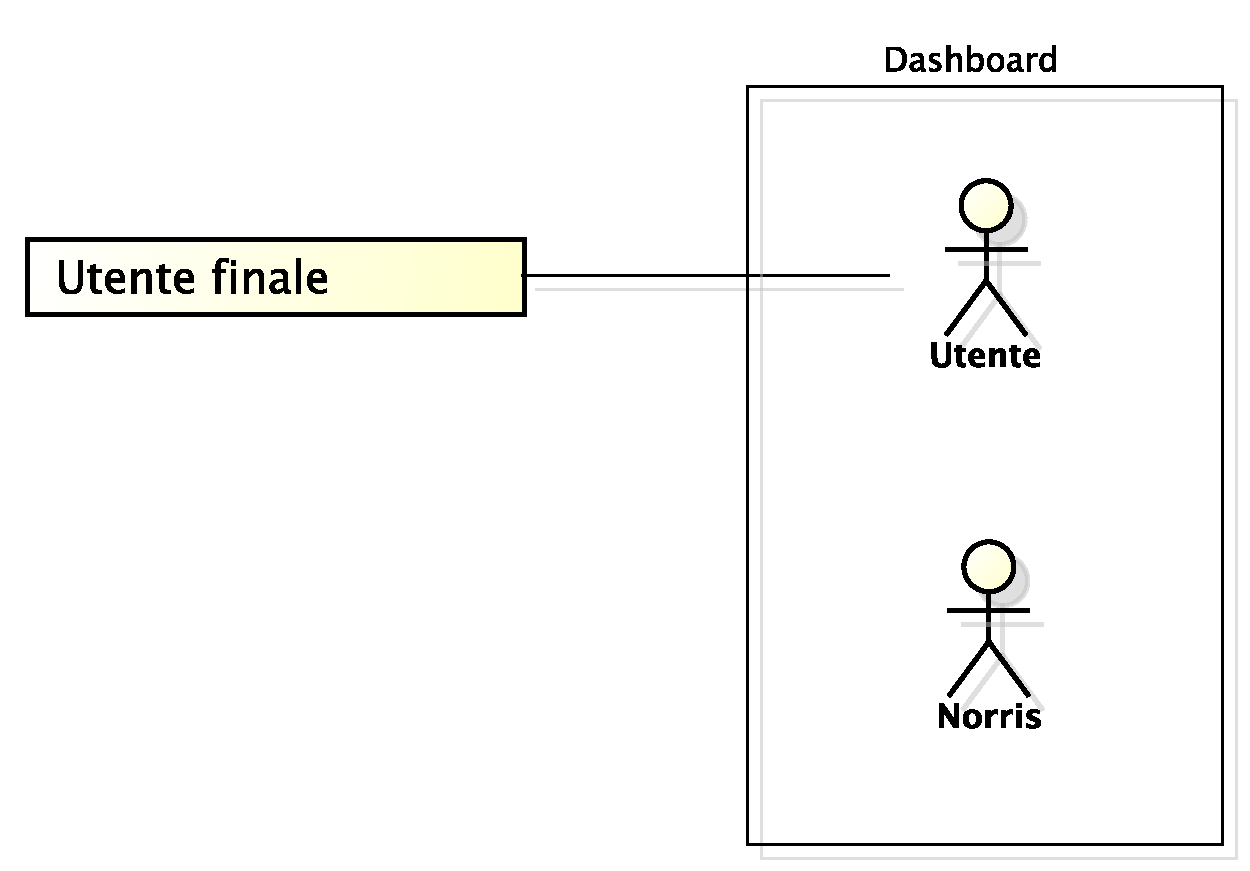
\includegraphics[scale=0.4]{Pics/UtentiAttoriDashboard}
		\caption{Dashboard - Relazione tra utenti e attori}
	\end{figure}
	\input{UseCase/UCD.tex}
